\section{Conclusiones}
\label{sec:conclusiones}

\subsection{Evaluación del proyecto}

La evaluación del proyecto en general es muy positiva, habiéndose cumplido sobradamente tanto con todos los objetivos iniciales como con los requisitos analizados.

Teniendo en cuenta los objetivos iniciales del proyecto y los requisito del mismo, lo más indicado habría sido utilizar únicamente una versión \textit{tiny} de YOLO, ya que fueron concebidas para ser explotados en dispositivos con pocos recursos. Se ha decidido implementar y entrenar modelos \textit{YOLO v3} para hacer una comparativa con su versión \textit{tiny}.

Todo el proyecto ha sido desarrollado en la plataforma \textit{Google Colab}, la cual presenta una serie de limitaciones en cuando a la capacidad del hardware disponible y en cuanto al tiempo de uso del mismo. Las limitaciones de capacidad del hardware han impactado al entrenamiento, teniendo que limitar tanto el tamaño de la red como el \textit{batch size} de la red. Las limitaciones de tiempo de uso han forzado realizar en varias fases el entrenamiento de los modelos, sobre todo los más grandes. En cada fase se ha realizado una \textit{transferencia de conocimiento}, teniendo como punto de partida el modelo resultante de la fase anterior, salvo en la fase inicial que se tiene como punto de partida el modelo entrenado publicado por los autores de \textit{YOLO}. Tras finalizar cada fase se ha realizado una evaluación del modelo obtenido y se ha comparado con el de la fase anterior para decidir si se prosigue con el entrenamiento.

Los modelos han sido entrenados pocas épocas debido a la cantidad de tiempo que requería el entrenamiento y por la limitación de tiempo de uso del hardware. La plataforma utilizada para el desarrollo del proyecto no está pensada para hacer un uso muy intensivo de la misma. Si es el caso y se lleva la infraestructura a sus límites, eres penalizado y las sucesivas solicitudes de hardware son rechazadas. Para el entrenamiento de varios de los modelos se ha llevado la plataforma al límite en repetidas ocasiones, haciendo uso de toda la capacidad de GPU (12 GB) y de todo el tiempo de uso disponible (12 horas). Así como en la fase inicial de entrenamiento era sencillo conseguir la asignación de recursos, en la fase final ha sido lo contrario, resultando difícil la asignación de recursos, teniendo que solicitarlos repetidas ocaciones durante varias horas hasta conseguirlos finalmente.

Al transformar los modelos a TFLite y evaluarlos desde python y java, los resultados obtenidos no son exactamente iguales. Existen pequeñas diferencias en las salidas del modelo a partir del 4-6 decimal. No se ha encontrado una explicación para esto, aunque estas diferencias no alteran demasiado las predicciones.

El tiempo de la inferencia en el dispositivo móvil ha resultado superior al esperado, obteniendo unos valores bajos de \textit{FPS} para las imágenes procesadas. Con un móvil de gama media (Nokia 7 plus) se alcanzan los 5-7 FPS. Con un móvil de gama alta (OnePlus 7 pro) se alcanzan unos 12 FPS.

\subsection{Alternativas y posibles mejoras que podrían haberse aplicado al proyecto (trabajos futuros)}

El principal punto de mejora se encuentra en los datos utilizados para el proyecto. Por un lado es un conjunto de datos un poco escaso y el etiquetado del mismo podría mejorarse. Con respecto al etiquetado, lo que se ha observado es que existen imágenes en las cuales hay baches que no han sido etiquetados. Para estos algoritmos es importante etiquetar todos los objetos a detectar existentes en la imagen.

Tras ver las diferencias de los resultados obtenidos con las imágenes originales y con las imágenes propias, se han observado notables diferencias en las características de los baches. En las imágenes originales los baches presentan priedras, arena, hojas. Sin embargo en los baches propios hay más asfalto, debido a que las carreteras son reasfaltadas, y los baches dejan al descubierto el asfalto original (ejemplo en figura \ref{fig:pothole_diffs}). Por lo que sería interesante disponer de un juego de datos obtenido en España para realizar el entrenamiento y ver cómo varían los resultados.

\begin{figure}[H]
	\centering
	\begin{subfigure}[h]{0.45\linewidth}
		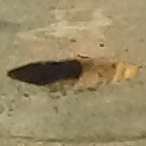
\includegraphics[width=\linewidth]{images/pothole_diff_orig.png}
	\end{subfigure}
	\begin{subfigure}[h]{0.45\linewidth}
		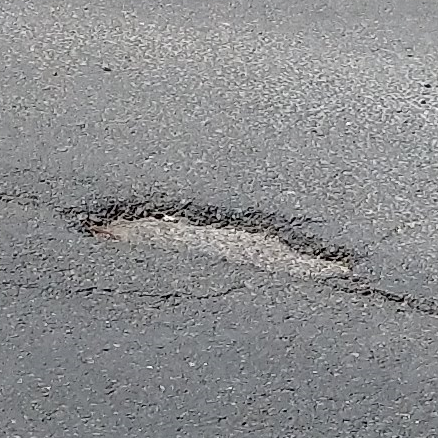
\includegraphics[width=\linewidth]{images/pothole_diff_esp.png}
	\end{subfigure}
	\caption{A la izquierda un ejemplo de bache típico presente en las imágenes originales. A la derecha un ejemplo de bache típico de las imágenes de España}
	\label{fig:pothole_diffs}
\end{figure}

Uno de los factores más determinantes para la precisión obtenida por los modelos ha sido el tamaño de los baches con respecto al de la imagen. Sería interesante disponer de un juego de datos en el que las fotos hayan sido tomadas desde el exterior del vehículo y con un encuadre de tal forma que los baches, aun siendo pequeños, tengan un tamaño representativo en la imagen. Esto podría conseguirse encuadrando la zona del asfalto frente al vehículo sin que aparezca paisaje al fondo ni en los laterales.

Otra vía de mejora a explorar para aumentar el número de \textit{FPS} procesadas por el modelo en el dispositivo móvil consistiría en realizar una transformación sobre el modelo para obtener uno \textit{quantized} \cite{s8_quantizedmodel}.

Habría que estar al tanto del soporte de GPU en \textit{TFLite} ya que actualmente se encuentra en fase experimental. Hoy en día es bastante frecuente que los dispositivos móviles tengan incorporada una GPU, por lo que sería muy interesante poder hacer uso de la misma. En la aplicación móvil se ha hecho uso de la misma, aunque no se ha obtenido una mejora, debido precisamente a que se encuentra en fase experimental y a que una de las operaciones del modelo (\textit{BatchNormalization}) \cite{s8_batchnormalization} no se encuentra soportada por el momento. Bien podría esperarse a que se soporte esta operación o bien se podría estudiar hacer una variación del modelo para remplazar esta operación por otra soportada sin que se afecte a la precisión del mismo.

\subsection{Conclusiones personales}

Tamaño pequeño de los baches

{\color{red} \textbf{!!! TODO}}